\documentclass[12pt,a4paper]{article}
\usepackage[margin=2cm]{geometry}
\usepackage{amsmath,amssymb,amsfonts}
\usepackage{tikz}
\usetikzlibrary{patterns,arrows.meta,calc,angles,quotes,decorations.markings}
\usepackage{enumitem}
\usepackage{xcolor}
\usepackage{fancyhdr}
\usepackage{titlesec}
\usepackage{tcolorbox}

\definecolor{examblue}{RGB}{0,51,102}
\definecolor{examred}{RGB}{153,0,0}
\definecolor{solutionbox}{RGB}{240,248,255}

\pagestyle{fancy}
\fancyhf{}
\rhead{\textbf{Mechanics Module}}
\lhead{\textbf{Ultimate Past Paper 3}}
\rfoot{Page \thepage}

\titleformat{\section}{\Large\bfseries\color{examblue}}{}{0em}{}[\titlerule]
\titleformat{\subsection}{\large\bfseries\color{examred}}{}{0em}{}

\newtcolorbox{questionbox}[1][]{
    colback=solutionbox, colframe=examblue, boxrule=1.5pt, arc=3mm, #1
}
\newtcolorbox{mcqbox}{
    colback=white, colframe=examred, boxrule=1pt, arc=2mm, left=5mm, right=5mm
}

\begin{document}

\begin{titlepage}
    \centering
    \vspace*{2cm}
    {\Huge\bfseries\color{examblue}MECHANICS MODULE}\par
    \vspace{0.5cm}
    {\Large\bfseries ULTIMATE PAST PAPER 3}\par
    \vspace{1.5cm}
    {\large Examination Period: May (Main)}\par
    \vspace{0.5cm}
    \rule{\linewidth}{2pt}\par
    \vspace{1cm}
    {\Large Time Allowed: \textbf{2 hours}}\par
    \vspace{0.5cm}
    {\Large Total Marks: \textbf{100} (40\% of Module)}\par
    \vspace{1.5cm}
    \rule{\linewidth}{1pt}\par
    \vspace{1cm}
    {\large\bfseries INSTRUCTIONS TO CANDIDATES}\par
    \vspace{0.5cm}
    \begin{minipage}{0.8\linewidth}
        \begin{enumerate}[label=\textbf{\arabic*.},leftmargin=*]
            \item Answer ALL questions
            \item Section A: 6 Short Multiple Choice Questions (60 marks)
            \item Section B: 2 Long Multiple Choice Questions (40 marks)
            \item All questions are INSANELY challenging
            \item Calculators permitted (must not store text)
        \end{enumerate}
    \end{minipage}
    \vfill
    {\small University of Birmingham - School of Engineering}\par
\end{titlepage}

\newpage
\section*{SECTION A: SHORT MULTIPLE CHOICE QUESTIONS (60 Marks)}
{\large\itshape Answer all 6 questions. Each question carries 10 marks.}
\vspace{0.5cm}

\begin{questionbox}
\subsection*{Question A1: Non-Proportional Loading with Kinematic Hardening [10 marks]}
A material element follows kinematic hardening with yield stress $\sigma_y = 320\,\text{MPa}$ 
and hardening modulus $H' = 15\,\text{GPa}$. The element experiences non-proportional loading:
$(\sigma_x, \sigma_y, \tau_{xy})$: $(0,0,0) \to (400,0,0) \to (400,200,0) \to (0,200,150)\,\text{MPa}$

\begin{center}
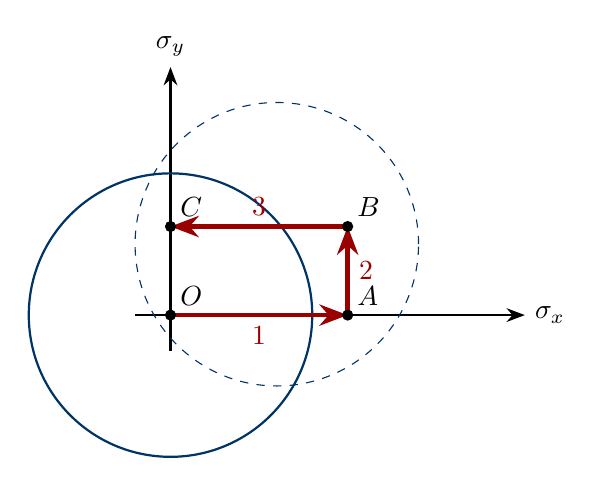
\begin{tikzpicture}[scale=0.9,>=Stealth]
    \draw[->,thick] (-0.5,0)--(5,0) node[right] {$\sigma_x$};
    \draw[->,thick] (0,-0.5)--(0,3.5) node[above] {$\sigma_y$};
    \draw[examblue,thick] (0,0) circle (2);
    \draw[examblue,dashed] (1.5,1) circle (2);
    \draw[examred,ultra thick,->] (0,0)--(2.5,0) node[midway,below] {1};
    \draw[examred,ultra thick,->] (2.5,0)--(2.5,1.25) node[midway,right] {2};
    \draw[examred,ultra thick,->] (2.5,1.25)--(0,1.25) node[midway,above] {3};
    \foreach \pt/\lbl in {(0,0)/O,(2.5,0)/A,(2.5,1.25)/B,(0,1.25)/C}
        \filldraw[black] \pt circle (2pt) node[above right] {$\lbl$};
\end{tikzpicture}
\end{center}

Using von Mises yield criterion with Prager's kinematic hardening rule, determine the 
accumulated equivalent plastic strain at the end of the loading path.

\begin{mcqbox}
\begin{enumerate}[label=(\Alph*),leftmargin=*]
    \item $\bar{\varepsilon}^p = 0.0087$
    \item $\bar{\varepsilon}^p = 0.0102$
    \item $\bar{\varepsilon}^p = 0.0078$
    \item $\bar{\varepsilon}^p = 0.0115$
    \item $\bar{\varepsilon}^p = 0.0094$
\end{enumerate}
\end{mcqbox}
\end{questionbox}

\begin{questionbox}
\subsection*{Question A2: Torsion of Thin-Walled Multi-Cell Sections [10 marks]}
The three-cell thin-walled section shown is subjected to torque $T = 45\,\text{kNm}$.
All walls have thickness $t = 6\,\text{mm}$ except central web ($t_w = 10\,\text{mm}$).
Outer cells $300\times400\,\text{mm}$, central cell $200\times400\,\text{mm}$. $G = 78\,\text{GPa}$.

\begin{center}
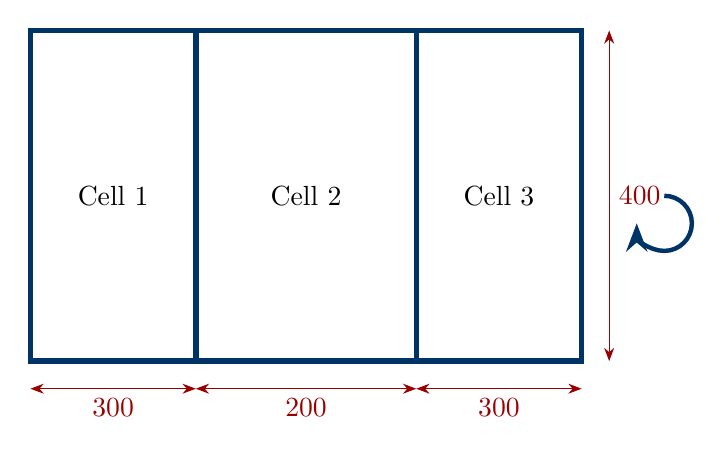
\begin{tikzpicture}[scale=0.7,>=Stealth]
    \draw[thick,examblue,line width=2pt] (0,0)--(10,0)--(10,6)--(0,6)--cycle;
    \draw[thick,examblue,line width=2pt] (3,0)--(3,6);
    \draw[thick,examblue,line width=2pt] (7,0)--(7,6);
    \node at (1.5,3) {Cell 1}; \node at (5,3) {Cell 2}; \node at (8.5,3) {Cell 3};
    \draw[<->,examred] (0,-0.5)--node[below]{$300$}(3,-0.5);
    \draw[<->,examred] (3,-0.5)--node[below]{$200$}(7,-0.5);
    \draw[<->,examred] (7,-0.5)--node[below]{$300$}(10,-0.5);
    \draw[<->,examred] (10.5,0)--node[right]{$400$}(10.5,6);
    \draw[->,examblue,ultra thick] (11.5,3) arc (90:-180:0.5);
\end{tikzpicture}
\end{center}

Accounting for warping restraint and shear flow compatibility, determine the maximum shear stress.

\begin{mcqbox}
\begin{enumerate}[label=(\Alph*),leftmargin=*]
    \item $\tau_{max} = 78.4\,\text{MPa}$
    \item $\tau_{max} = 85.7\,\text{MPa}$
    \item $\tau_{max} = 72.1\,\text{MPa}$
    \item $\tau_{max} = 91.3\,\text{MPa}$
    \item $\tau_{max} = 81.9\,\text{MPa}$
\end{enumerate}
\end{mcqbox}
\end{questionbox}

\begin{questionbox}
\subsection*{Question A3: Column Buckling with Elastic Restraints [10 marks]}
A steel column ($E = 200\,\text{GPa}$, $I = 42\times10^6\,\text{mm}^4$, $L = 5.5\,\text{m}$) 
is pinned at base with rotational spring $k_\theta = 8500\,\text{kNm/rad}$ and lateral spring 
$k_h = 12000\,\text{kN/m}$ at top.

\begin{center}
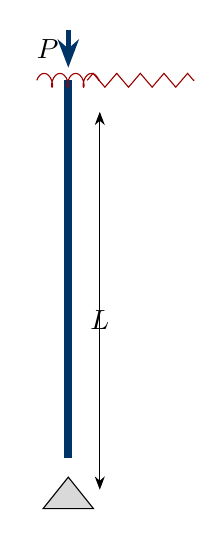
\begin{tikzpicture}[scale=0.8,>=Stealth]
    \draw[thick,examblue,line width=3pt] (0,0)--(0,6);
    \draw[fill=gray!30] (0,-0.3)--++(-0.4,-0.5)--++(0.8,0)--cycle;
    \draw[examred,decorate,decoration={coil,segment length=2mm}] (-0.5,6)--(0.5,6);
    \draw[examred,decorate,decoration={zigzag,segment length=3mm}] (0.3,6)--(2,6);
    \draw[->,examblue,ultra thick] (0,6.8)--(0,6.2);
    \node[left] at (0,6.5) {$P$};
    \draw[<->] (0.5,-0.5)--node[below]{$L$}(0.5,5.5);
\end{tikzpicture}
\end{center}

Solving the transcendental buckling equation, determine the critical buckling load $P_{cr}$.

\begin{mcqbox}
\begin{enumerate}[label=(\Alph*),leftmargin=*]
    \item $P_{cr} = 2847\,\text{kN}$
    \item $P_{cr} = 3156\,\text{kN}$
    \item $P_{cr} = 2634\,\text{kN}$
    \item $P_{cr} = 3421\,\text{kN}$
    \item $P_{cr} = 2978\,\text{kN}$
\end{enumerate}
\end{mcqbox}
\end{questionbox}

\begin{questionbox}
\subsection*{Question A4: Lagrangian Dynamics of Coupled Systems [10 marks]}
Double pendulum-cart system: cart mass $M = 80\,\text{kg}$, links ($m_1 = 25\,\text{kg}$, $L_1 = 1.8\,\text{m}$) 
and ($m_2 = 18\,\text{kg}$, $L_2 = 1.4\,\text{m}$). Cart attached to spring $k = 4500\,\text{N/m}$ 
and damper $c = 180\,\text{Ns/m}$.

\begin{center}
\begin{tikzpicture}[scale=0.8,>=Stealth]
    \draw[thick] (-1,0)--(7,0);
    \draw[thick,examblue,fill=gray!30] (2,0) rectangle (3.5,0.8);
    \draw[examred,decorate,decoration={zigzag,segment length=2mm}] (0,0.4)--(2,0.4);
    \draw[thick,examblue,line width=2pt] (2.75,0.8)--(3.5,2.2);
    \draw[thick,examred,line width=2pt] (3.5,2.2)--(4.3,3.4);
    \pic["$\theta_1$",draw] {angle={(3.5,0.8)--(2.75,0.8)--(3.5,2.2)}};
    \pic["$\theta_2$",draw] {angle={(4.3,2.2)--(3.5,2.2)--(4.3,3.4)}};
\end{tikzpicture}
\end{center}

Using Lagrange's equations linearized about vertical equilibrium, determine the lowest natural frequency.

\begin{mcqbox}
\begin{enumerate}[label=(\Alph*),leftmargin=*]
    \item $\omega_1 = 1.87\,\text{rad/s}$
    \item $\omega_1 = 2.14\,\text{rad/s}$
    \item $\omega_1 = 1.63\,\text{rad/s}$
    \item $\omega_1 = 2.45\,\text{rad/s}$
    \item $\omega_1 = 1.95\,\text{rad/s}$
\end{enumerate}
\end{mcqbox}
\end{questionbox}

\begin{questionbox}
\subsection*{Question A5: Mixed-Mode Fracture [10 marks]}
Angled crack $2a = 24\,\text{mm}$ at $\beta = 40^\circ$ in infinite plate under biaxial loading 
($\sigma_1 = 180\,\text{MPa}$, $\sigma_2 = -65\,\text{MPa}$).

\begin{center}
\begin{tikzpicture}[scale=0.9,>=Stealth]
    \draw[thick,examblue] (-3,-2)--(3,-2)--(3,2)--(-3,2)--cycle;
    \draw[examred,ultra thick] (-1,-0.84)--(1,0.84);
    \draw[->,examblue] (-3.2,1)--(-2.5,1); \draw[->,examblue] (3.2,1)--(2.5,1);
    \pic["$\beta$",draw] {angle={(1,0)--(0,0)--(1,0.84)}};
    \draw[<->,examred] (-1,-1.1)--node[below]{$2a$}(1,-1.1);
\end{tikzpicture}
\end{center}

With $K_I = \sigma\sqrt{\pi a}\sin^2\beta$, $K_{II} = \sigma\sqrt{\pi a}\sin\beta\cos\beta$, 
determine $K_{eff} = \sqrt{K_I^2 + 3K_{II}^2}$.

\begin{mcqbox}
\begin{enumerate}[label=(\Alph*),leftmargin=*]
    \item $K_{eff} = 42.7\,\text{MPa}\sqrt{\text{m}}$
    \item $K_{eff} = 48.3\,\text{MPa}\sqrt{\text{m}}$
    \item $K_{eff} = 38.9\,\text{MPa}\sqrt{\text{m}}$
    \item $K_{eff} = 52.1\,\text{MPa}\sqrt{\text{m}}$
    \item $K_{eff} = 45.6\,\text{MPa}\sqrt{\text{m}}$
\end{enumerate}
\end{mcqbox}
\end{questionbox}

\begin{questionbox}
\subsection*{Question A6: Wave Propagation with Dispersion [10 marks]}
Steel rod ($E = 200\,\text{GPa}$, $\rho = 7850\,\text{kg/m}^3$, $d = 25\,\text{mm}$, $L = 3\,\text{m}$) 
fixed at one end, impacted by mass $M = 15\,\text{kg}$ at $v_0 = 8\,\text{m/s}$.

\begin{center}
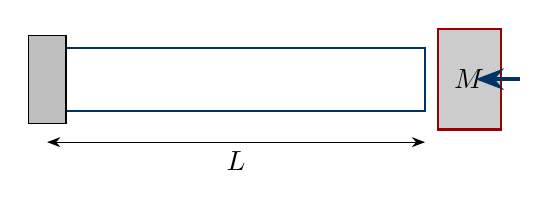
\begin{tikzpicture}[scale=0.8,>=Stealth]
    \draw[thick,examblue] (0,-0.5) rectangle (6,0.5);
    \draw[fill=gray!50] (-0.3,-0.7) rectangle (0.3,0.7);
    \draw[thick,examred,fill=gray!40] (6.2,-0.8) rectangle (7.2,0.8);
    \node at (6.7,0) {$M$};
    \draw[->,examblue,ultra thick] (7.5,0)--(6.8,0);
    \draw[<->] (0,-1)--node[below]{$L$}(6,-1);
\end{tikzpicture}
\end{center}

Accounting for Love-Rayleigh dispersion, determine maximum impact force with first reflection.

\begin{mcqbox}
\begin{enumerate}[label=(\Alph*),leftmargin=*]
    \item $F_{max} = 187\,\text{kN}$
    \item $F_{max} = 203\,\text{kN}$
    \item $F_{max} = 174\,\text{kN}$
    \item $F_{max} = 218\,\text{kN}$
    \item $F_{max} = 195\,\text{kN}$
\end{enumerate}
\end{mcqbox}
\end{questionbox}

\newpage
\section*{SECTION B: LONG MULTIPLE CHOICE QUESTIONS (40 Marks)}
{\large\itshape Answer both questions. Each question carries 20 marks.}
\vspace{0.5cm}

\begin{questionbox}
\subsection*{Question B1: Elasto-Plastic Thick-Walled Cylinder [20 marks]}
Thick cylinder ($a = 100\,\text{mm}$, $b = 180\,\text{mm}$) with $\sigma_y = 420\,\text{MPa}$, 
$E = 200\,\text{GPa}$, $\nu = 0.3$. Internal pressure causes plastic zone to $c = 140\,\text{mm}$.

\begin{center}
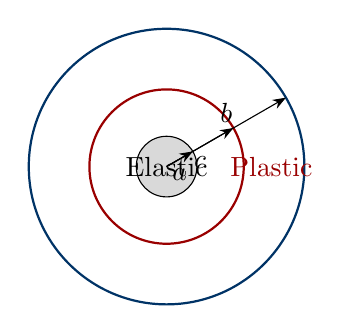
\begin{tikzpicture}[scale=0.7,>=Stealth]
    \draw[thick,examblue] (0,0) circle (2.5);
    \draw[thick,examred] (0,0) circle (1.4);
    \draw[fill=gray!30] (0,0) circle (0.55);
    \draw[->] (0,0)--(30:2.5) node[midway,above] {$b$};
    \draw[->] (0,0)--(30:1.4) node[midway,below] {$c$};
    \draw[->] (0,0)--(30:0.55) node[midway,below] {$a$};
    \node at (0,0) {Elastic}; \node[examred] at (1.9,0) {Plastic};
\end{tikzpicture}
\end{center}

Using Tresca criterion with residual stresses upon unloading, determine autofrettage benefit ratio.

\begin{mcqbox}
\begin{enumerate}[label=(\Alph*),leftmargin=*]
    \item Ratio = 2.14
    \item Ratio = 2.47
    \item Ratio = 1.89
    \item Ratio = 2.63
    \item Ratio = 2.31
\end{enumerate}
\end{mcqbox}
\end{questionbox}

\begin{questionbox}
\subsection*{Question B2: Dynamic Plate Response to Blast [20 marks]}
Rectangular plate ($a = 1.2\,\text{m}$, $b = 0.8\,\text{m}$, $h = 12\,\text{mm}$) simply supported.
$E = 200\,\text{GPa}$, $\nu = 0.3$, $\rho = 7850\,\text{kg/m}^3$, $\sigma_y = 350\,\text{MPa}$.
Blast pressure: $p(t) = p_0 e^{-t/\tau}\sin(\pi x/a)\sin(\pi y/b)$ with $p_0 = 150\,\text{kPa}$, $\tau = 8\,\text{ms}$.

\begin{center}
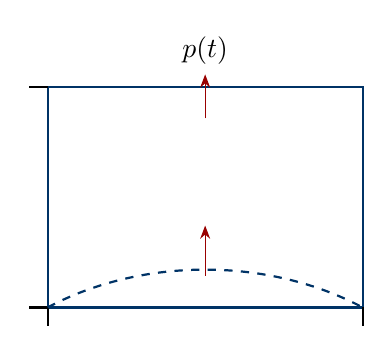
\begin{tikzpicture}[scale=0.8,>=Stealth]
    \draw[thick,examblue] (0,0)--(5,0)--(5,3.5)--(0,3.5)--cycle;
    \foreach \x in {0,5} \draw[thick] (\x,0)--++(0,-0.3);
    \foreach \y in {0,3.5} \draw[thick] (0,\y)--++(-0.3,0);
    \draw[examred,->] (2.5,0.5)--(2.5,1.3); \draw[examred,->] (2.5,3)--(2.5,3.7);
    \node[above] at (2.5,3.7) {$p(t)$};
    \draw[examblue,dashed,thick] (0,0)..controls(1.5,0.8)and(3.5,0.8)..(5,0);
\end{tikzpicture}
\end{center}

Using modal analysis with Duhamel's integral and membrane action, determine maximum dynamic deflection.

\begin{mcqbox}
\begin{enumerate}[label=(\Alph*),leftmargin=*]
    \item $w_{max} = 18.7\,\text{mm}$
    \item $w_{max} = 22.4\,\text{mm}$
    \item $w_{max} = 16.3\,\text{mm}$
    \item $w_{max} = 25.1\,\text{mm}$
    \item $w_{max} = 20.5\,\text{mm}$
\end{enumerate}
\end{mcqbox}
\end{questionbox}

\end{document}
